\documentclass[../main]{subfiles}

\questiontrue
\solutiontrue

\begin{document}
    \ifquestion

    \section{Charge-Coupled Device}

\parte{A}{A Bit of Quantum Mechanics}

As mentioned in question 14, Nill continued his optical studies with the analysis of CCD operation. The CCD, which stands for \textit{Charge-Coupled Device}, is a photosensitive device capable of converting the received radiation into electric charge. A CCD is composed of cells (pixels) that absorb radiation and use the energy of incident photons to release electrons from a semiconductor and move them to a transfer zone that confines the particles in a potential well. The charge is then transferred to an adjacent cell, recursively, until it reaches the reader at the edge of the device, as shown in the diagram below:
    
    \begin{figure}[htpb]
    \centering
    
    \tikzset{every picture/.style={line width=0.75pt}} %set default line width to 0.75pt        

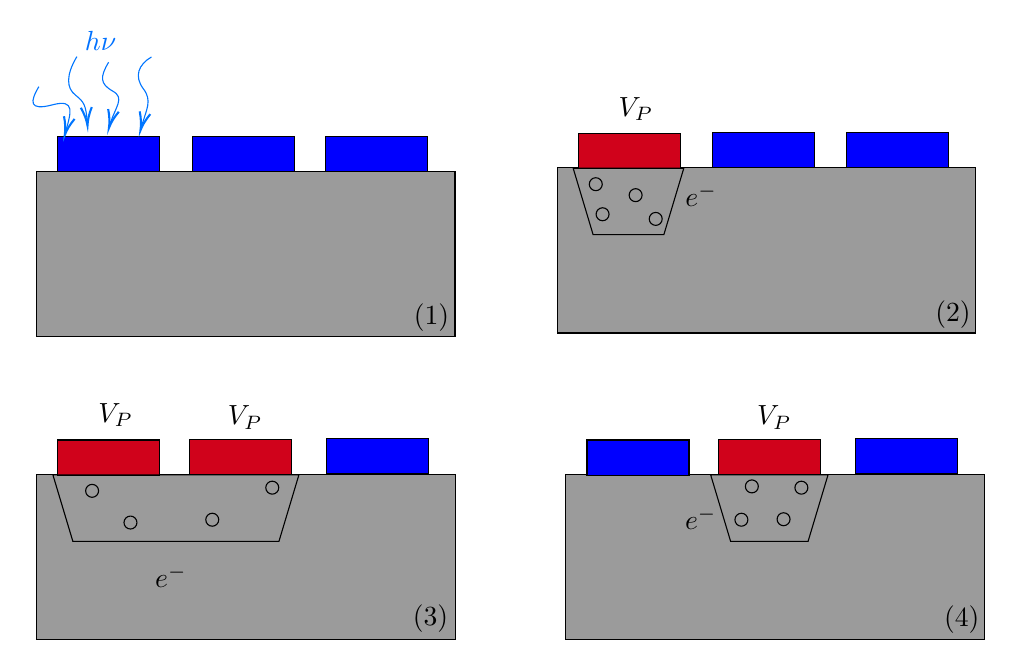
\begin{tikzpicture}[x=0.75pt,y=0.75pt,yscale=-0.8,xscale=0.8]
%uncomment if require: \path (0,598); %set diagram left start at 0, and has height of 598

%Shape: Rectangle [id:dp7762740638109957] 
\draw  [fill={rgb, 255:red, 155; green, 155; blue, 155 }  ,fill opacity=1 ] (51,101) -- (303,101) -- (303,200.5) -- (51,200.5) -- cycle ;
%Shape: Rectangle [id:dp36389541235280687] 
\draw  [color={rgb, 255:red, 0; green, 0; blue, 0 }  ,draw opacity=1 ][fill={rgb, 255:red, 0; green, 0; blue, 255 }  ,fill opacity=1 ] (63.6,79.8) -- (125,79.8) -- (125,101) -- (63.6,101) -- cycle ;
%Shape: Rectangle [id:dp3049043096290862] 
\draw  [fill={rgb, 255:red, 0; green, 0; blue, 255 }  ,fill opacity=1 ] (144.8,79.8) -- (206.2,79.8) -- (206.2,101) -- (144.8,101) -- cycle ;
%Shape: Rectangle [id:dp5476143105060063] 
\draw  [fill={rgb, 255:red, 0; green, 0; blue, 255 }  ,fill opacity=1 ] (225.2,79.8) -- (286.6,79.8) -- (286.6,101) -- (225.2,101) -- cycle ;
%Curve Lines [id:da7729616330017184] 
\draw [color={rgb, 255:red, 0; green, 115; blue, 255 }  ,draw opacity=1 ]   (94.4,35.3) .. controls (89.2,44.1) and (89.1,48.3) .. (96.95,52.7) .. controls (104.41,56.88) and (98.46,61.96) .. (95.11,73.09) ;
\draw [shift={(94.6,74.9)}, rotate = 284.47] [color={rgb, 255:red, 0; green, 115; blue, 255 }  ,draw opacity=1 ][line width=0.75]    (10.93,-3.29) .. controls (6.95,-1.4) and (3.31,-0.3) .. (0,0) .. controls (3.31,0.3) and (6.95,1.4) .. (10.93,3.29)   ;
%Curve Lines [id:da09713896278494616] 
\draw [color={rgb, 255:red, 0; green, 118; blue, 255 }  ,draw opacity=1 ]   (75.3,31.9) .. controls (68.5,43.3) and (69.1,50.9) .. (74.45,55.1) .. controls (79.51,59.07) and (80.77,60.89) .. (81.56,71.46) ;
\draw [shift={(81.7,73.4)}, rotate = 266.28] [color={rgb, 255:red, 0; green, 118; blue, 255 }  ,draw opacity=1 ][line width=0.75]    (10.93,-3.29) .. controls (6.95,-1.4) and (3.31,-0.3) .. (0,0) .. controls (3.31,0.3) and (6.95,1.4) .. (10.93,3.29)   ;
%Curve Lines [id:da18686819886068862] 
\draw [color={rgb, 255:red, 0; green, 117; blue, 255 }  ,draw opacity=1 ]   (120.2,32.1) .. controls (112.4,36.7) and (109.6,43.7) .. (115.35,51.3) .. controls (120.82,58.52) and (117.21,63.39) .. (114.09,74.49) ;
\draw [shift={(113.6,76.3)}, rotate = 284.47] [color={rgb, 255:red, 0; green, 117; blue, 255 }  ,draw opacity=1 ][line width=0.75]    (10.93,-3.29) .. controls (6.95,-1.4) and (3.31,-0.3) .. (0,0) .. controls (3.31,0.3) and (6.95,1.4) .. (10.93,3.29)   ;
%Curve Lines [id:da33926080997391916] 
\draw [color={rgb, 255:red, 0; green, 117; blue, 255 }  ,draw opacity=1 ]   (52.4,50) .. controls (47.2,58.8) and (46,64.8) .. (60.75,60.9) .. controls (74.77,57.2) and (71.58,65.85) .. (68.49,77.36) ;
\draw [shift={(68,79.2)}, rotate = 284.47] [color={rgb, 255:red, 0; green, 117; blue, 255 }  ,draw opacity=1 ][line width=0.75]    (10.93,-3.29) .. controls (6.95,-1.4) and (3.31,-0.3) .. (0,0) .. controls (3.31,0.3) and (6.95,1.4) .. (10.93,3.29)   ;
%Shape: Rectangle [id:dp5809119219422243] 
\draw  [fill={rgb, 255:red, 155; green, 155; blue, 155 }  ,fill opacity=1 ] (364.5,98.83) -- (616.5,98.83) -- (616.5,198.33) -- (364.5,198.33) -- cycle ;
%Shape: Rectangle [id:dp07440922504317338] 
\draw  [fill={rgb, 255:red, 0; green, 0; blue, 255 }  ,fill opacity=1 ] (458.3,77.63) -- (519.7,77.63) -- (519.7,98.83) -- (458.3,98.83) -- cycle ;
%Shape: Rectangle [id:dp16800968988931153] 
\draw  [fill={rgb, 255:red, 0; green, 0; blue, 255 }  ,fill opacity=1 ] (538.7,77.63) -- (600.1,77.63) -- (600.1,98.83) -- (538.7,98.83) -- cycle ;
%Shape: Rectangle [id:dp6984118990371031] 
\draw  [fill={rgb, 255:red, 208; green, 2; blue, 27 }  ,fill opacity=1 ] (377.2,78.13) -- (438.6,78.13) -- (438.6,99.33) -- (377.2,99.33) -- cycle ;
%Shape: Trapezoid [id:dp7422125318413455] 
\draw   (440.8,99.13) -- (428.8,139.13) -- (386.2,139.13) -- (374.2,99.13) -- cycle ;
%Shape: Circle [id:dp39898352833087447] 
\draw   (383.9,108.73) .. controls (383.9,106.58) and (385.65,104.83) .. (387.8,104.83) .. controls (389.95,104.83) and (391.7,106.58) .. (391.7,108.73) .. controls (391.7,110.89) and (389.95,112.63) .. (387.8,112.63) .. controls (385.65,112.63) and (383.9,110.89) .. (383.9,108.73) -- cycle ;
%Shape: Circle [id:dp33179528118226775] 
\draw   (420,129.63) .. controls (420,127.48) and (421.75,125.73) .. (423.9,125.73) .. controls (426.05,125.73) and (427.8,127.48) .. (427.8,129.63) .. controls (427.8,131.79) and (426.05,133.53) .. (423.9,133.53) .. controls (421.75,133.53) and (420,131.79) .. (420,129.63) -- cycle ;
%Shape: Circle [id:dp933396918757815] 
\draw   (388,126.83) .. controls (388,124.68) and (389.75,122.93) .. (391.9,122.93) .. controls (394.05,122.93) and (395.8,124.68) .. (395.8,126.83) .. controls (395.8,128.99) and (394.05,130.73) .. (391.9,130.73) .. controls (389.75,130.73) and (388,128.99) .. (388,126.83) -- cycle ;
%Shape: Circle [id:dp02732893684295501] 
\draw   (407.9,115.33) .. controls (407.9,113.18) and (409.65,111.43) .. (411.8,111.43) .. controls (413.95,111.43) and (415.7,113.18) .. (415.7,115.33) .. controls (415.7,117.49) and (413.95,119.23) .. (411.8,119.23) .. controls (409.65,119.23) and (407.9,117.49) .. (407.9,115.33) -- cycle ;
%Shape: Rectangle [id:dp09121840260450975] 
\draw  [fill={rgb, 255:red, 155; green, 155; blue, 155 }  ,fill opacity=1 ] (51.17,283.5) -- (303.17,283.5) -- (303.17,383) -- (51.17,383) -- cycle ;
%Shape: Rectangle [id:dp700871054788397] 
\draw  [fill={rgb, 255:red, 0; green, 0; blue, 255 }  ,fill opacity=1 ] (225.65,262.01) -- (287.05,262.01) -- (287.05,283.21) -- (225.65,283.21) -- cycle ;
%Shape: Rectangle [id:dp28459690046053665] 
\draw  [fill={rgb, 255:red, 208; green, 2; blue, 27 }  ,fill opacity=1 ] (63.87,262.8) -- (125.27,262.8) -- (125.27,284) -- (63.87,284) -- cycle ;
%Shape: Trapezoid [id:dp2860569593256348] 
\draw   (209,283.8) -- (197,323.8) -- (72.87,323.8) -- (60.87,283.8) -- cycle ;
%Shape: Circle [id:dp6029768715322994] 
\draw   (80.57,293.4) .. controls (80.57,291.25) and (82.31,289.5) .. (84.47,289.5) .. controls (86.62,289.5) and (88.37,291.25) .. (88.37,293.4) .. controls (88.37,295.55) and (86.62,297.3) .. (84.47,297.3) .. controls (82.31,297.3) and (80.57,295.55) .. (80.57,293.4) -- cycle ;
%Shape: Circle [id:dp27898771504330644] 
\draw   (152.93,310.8) .. controls (152.93,308.65) and (154.68,306.9) .. (156.83,306.9) .. controls (158.99,306.9) and (160.73,308.65) .. (160.73,310.8) .. controls (160.73,312.95) and (158.99,314.7) .. (156.83,314.7) .. controls (154.68,314.7) and (152.93,312.95) .. (152.93,310.8) -- cycle ;
%Shape: Circle [id:dp1167938415043257] 
\draw   (103.67,312.5) .. controls (103.67,310.35) and (105.41,308.6) .. (107.57,308.6) .. controls (109.72,308.6) and (111.47,310.35) .. (111.47,312.5) .. controls (111.47,314.65) and (109.72,316.4) .. (107.57,316.4) .. controls (105.41,316.4) and (103.67,314.65) .. (103.67,312.5) -- cycle ;
%Shape: Circle [id:dp41030766978712685] 
\draw   (189.07,291.5) .. controls (189.07,289.35) and (190.81,287.6) .. (192.97,287.6) .. controls (195.12,287.6) and (196.87,289.35) .. (196.87,291.5) .. controls (196.87,293.65) and (195.12,295.4) .. (192.97,295.4) .. controls (190.81,295.4) and (189.07,293.65) .. (189.07,291.5) -- cycle ;
%Shape: Rectangle [id:dp07442625823416726] 
\draw  [fill={rgb, 255:red, 208; green, 2; blue, 27 }  ,fill opacity=1 ] (143.1,262.23) -- (204.5,262.23) -- (204.5,283.43) -- (143.1,283.43) -- cycle ;
%Shape: Rectangle [id:dp2422305128253972] 
\draw  [fill={rgb, 255:red, 155; green, 155; blue, 155 }  ,fill opacity=1 ] (369.83,283.5) -- (621.83,283.5) -- (621.83,383) -- (369.83,383) -- cycle ;
%Shape: Rectangle [id:dp1679167051167325] 
\draw  [fill={rgb, 255:red, 0; green, 0; blue, 255 }  ,fill opacity=1 ] (544.32,262.01) -- (605.72,262.01) -- (605.72,283.21) -- (544.32,283.21) -- cycle ;
%Shape: Rectangle [id:dp6470125547435854] 
\draw  [fill={rgb, 255:red, 0; green, 0; blue, 255 }  ,fill opacity=1 ] (382.53,262.8) -- (443.93,262.8) -- (443.93,284) -- (382.53,284) -- cycle ;
%Shape: Trapezoid [id:dp9166119573516835] 
\draw   (527.67,283.8) -- (515.67,323.8) -- (469,323.8) -- (457,283.8) -- cycle ;
%Shape: Circle [id:dp37841417633613816] 
\draw   (477.9,290.73) .. controls (477.9,288.58) and (479.65,286.83) .. (481.8,286.83) .. controls (483.95,286.83) and (485.7,288.58) .. (485.7,290.73) .. controls (485.7,292.89) and (483.95,294.63) .. (481.8,294.63) .. controls (479.65,294.63) and (477.9,292.89) .. (477.9,290.73) -- cycle ;
%Shape: Circle [id:dp03911513112668308] 
\draw   (471.6,310.8) .. controls (471.6,308.65) and (473.35,306.9) .. (475.5,306.9) .. controls (477.65,306.9) and (479.4,308.65) .. (479.4,310.8) .. controls (479.4,312.95) and (477.65,314.7) .. (475.5,314.7) .. controls (473.35,314.7) and (471.6,312.95) .. (471.6,310.8) -- cycle ;
%Shape: Circle [id:dp29760600950145366] 
\draw   (497,310.5) .. controls (497,308.35) and (498.75,306.6) .. (500.9,306.6) .. controls (503.05,306.6) and (504.8,308.35) .. (504.8,310.5) .. controls (504.8,312.65) and (503.05,314.4) .. (500.9,314.4) .. controls (498.75,314.4) and (497,312.65) .. (497,310.5) -- cycle ;
%Shape: Circle [id:dp5365769637021729] 
\draw   (507.73,291.5) .. controls (507.73,289.35) and (509.48,287.6) .. (511.63,287.6) .. controls (513.79,287.6) and (515.53,289.35) .. (515.53,291.5) .. controls (515.53,293.65) and (513.79,295.4) .. (511.63,295.4) .. controls (509.48,295.4) and (507.73,293.65) .. (507.73,291.5) -- cycle ;
%Shape: Rectangle [id:dp06151471045084267] 
\draw  [fill={rgb, 255:red, 208; green, 2; blue, 27 }  ,fill opacity=1 ] (461.77,262.23) -- (523.17,262.23) -- (523.17,283.43) -- (461.77,283.43) -- cycle ;

% Text Node
\draw (78.6,14.8) node [anchor=north west][inner sep=0.75pt]  [color={rgb, 255:red, 0; green, 113; blue, 255 }  ,opacity=1 ]  {$h\nu $};
% Text Node
\draw (440.2,107.17) node [anchor=north west][inner sep=0.75pt]    {$e^{-}$};
% Text Node
\draw (400,54.73) node [anchor=north west][inner sep=0.75pt]    {$V_{P}$};
% Text Node
\draw (120.87,336.51) node [anchor=north west][inner sep=0.75pt]    {$e^{-}$};
% Text Node
\draw (86.67,239.4) node [anchor=north west][inner sep=0.75pt]    {$V_{P}$};
% Text Node
\draw (164.67,240.73) node [anchor=north west][inner sep=0.75pt]    {$V_{P}$};
% Text Node
\draw (440,301.84) node [anchor=north west][inner sep=0.75pt]    {$e^{-}$};
% Text Node
\draw (483.33,240.73) node [anchor=north west][inner sep=0.75pt]    {$V_{P}$};
% Text Node
\draw (276.67,179.07) node [anchor=north west][inner sep=0.75pt]    {$( 1)$};
% Text Node
\draw (276,360.4) node [anchor=north west][inner sep=0.75pt]    {$( 3)$};
% Text Node
\draw (596,361.07) node [anchor=north west][inner sep=0.75pt]    {$( 4)$};
% Text Node
\draw (590.67,177.07) node [anchor=north west][inner sep=0.75pt]    {$( 2)$};


\end{tikzpicture}
    
\caption{Operating principle of energy storage in the CCD and the movement of photon-electrons through the CCD \emph{array}}
\end{figure}

In this problem, we will analyze the effect caused by the storage of electrons in the potential well generated by the CCD's capacitors and how, due to quantum effects, the charge can escape and be lost.

For this, we will use a simplified model where each incident photon with energy greater than $E_{\phi}$, the energy between the conduction and valence bands of the semiconductor\footnote{Commonly known as the \textit{Band Gap}}, excites an electron with energy equivalent to $E_\phi$. Consider that any excess energy is lost as thermal energy in the material.

\ut{A.1} Silicon is a semiconductor material commonly used in this type of device. It has a \textit{band gap} of approximately $1.1$ eV. Calculate the largest wavelength that can be detected by a CCD made of silicon.

\begin{doublespace}



\end{doublespace}

In this model, the potential well has energy $V_P<E_\phi$, while the surrounding region has energy $V_0>E_\phi$, as shown in the figure below, for the $x$ axis:
    
    \begin{figure}[htpb]
    \centering
    
\tikzset{every picture/.style={line width=0.75pt}} %set default line width to 0.75pt        

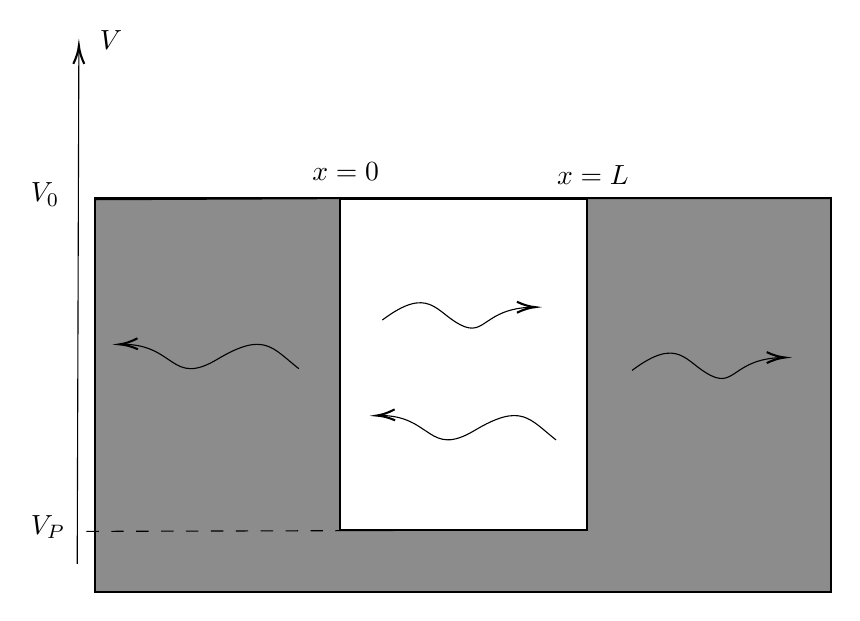
\begin{tikzpicture}[x=0.75pt,y=0.75pt,yscale=-0.8,xscale=0.8]
%uncomment if require: \path (0,598); %set diagram left start at 0, and has height of 598

%Shape: Rectangle [id:dp38555278635247947] 
\draw  [fill={rgb, 255:red, 140; green, 140; blue, 140 }  ,fill opacity=1 ][line width=0.75]  (102,415.77) -- (545.5,415.77) -- (545.5,178.6) -- (102,178.6) -- cycle ;
%Straight Lines [id:da29479573694631456] 
\draw    (102,179.35) -- (249.67,178.68) ;
%Straight Lines [id:da3629064810898259] 
\draw    (249.67,178.68) -- (249.67,378.68) ;
%Straight Lines [id:da5045979724920169] 
\draw    (249.67,378.68) -- (398,378.02) ;
%Straight Lines [id:da6355524656716758] 
\draw    (545.5,178.6) -- (398.33,178.68) ;
%Straight Lines [id:da677481002613953] 
\draw    (398.33,178.68) -- (398,378.02) ;
%Straight Lines [id:da629295192086939] 
\draw    (91.5,398.6) -- (92.49,88.6) ;
\draw [shift={(92.5,86.6)}, rotate = 90.18] [color={rgb, 255:red, 0; green, 0; blue, 0 }  ][line width=0.75]    (10.93,-3.29) .. controls (6.95,-1.4) and (3.31,-0.3) .. (0,0) .. controls (3.31,0.3) and (6.95,1.4) .. (10.93,3.29)   ;
%Straight Lines [id:da935220847793578] 
\draw  [dash pattern={on 4.5pt off 4.5pt}]  (97,379.1) -- (249.67,378.68) ;
%Curve Lines [id:da17698222665796814] 
\draw    (225,281.13) .. controls (208.78,268.46) and (204.33,258.46) .. (175.83,275.48) .. controls (147.9,292.15) and (150.76,266.42) .. (118.99,266.43) ;
\draw [shift={(117,266.46)}, rotate = 358.12] [color={rgb, 255:red, 0; green, 0; blue, 0 }  ][line width=0.75]    (10.93,-3.29) .. controls (6.95,-1.4) and (3.31,-0.3) .. (0,0) .. controls (3.31,0.3) and (6.95,1.4) .. (10.93,3.29)   ;
%Curve Lines [id:da045633886727725725] 
\draw    (425.67,282.14) .. controls (453.99,260.9) and (457.71,277.49) .. (472.92,285.14) .. controls (487.82,292.65) and (486.72,275.24) .. (515.85,274.42) ;
\draw [shift={(517.67,274.39)}, rotate = 179.77] [color={rgb, 255:red, 0; green, 0; blue, 0 }  ][line width=0.75]    (10.93,-3.29) .. controls (6.95,-1.4) and (3.31,-0.3) .. (0,0) .. controls (3.31,0.3) and (6.95,1.4) .. (10.93,3.29)   ;
%Shape: Rectangle [id:dp17530728785151495] 
\draw  [fill={rgb, 255:red, 255; green, 255; blue, 255 }  ,fill opacity=1 ][line width=0.75]  (249.67,378.35) -- (398.33,378.35) -- (398.33,178.68) -- (249.67,178.68) -- cycle ;
%Curve Lines [id:da5059885877555934] 
\draw    (275.25,251.81) .. controls (303.57,230.57) and (307.3,247.15) .. (322.5,254.81) .. controls (337.4,262.31) and (336.3,244.91) .. (365.43,244.09) ;
\draw [shift={(367.25,244.06)}, rotate = 179.77] [color={rgb, 255:red, 0; green, 0; blue, 0 }  ][line width=0.75]    (10.93,-3.29) .. controls (6.95,-1.4) and (3.31,-0.3) .. (0,0) .. controls (3.31,0.3) and (6.95,1.4) .. (10.93,3.29)   ;
%Curve Lines [id:da2681729615357309] 
\draw    (379.89,324.02) .. controls (363.67,311.35) and (359.22,301.35) .. (330.72,318.37) .. controls (302.79,335.04) and (305.11,309.09) .. (273.85,309.31) ;
\draw [shift={(271.89,309.35)}, rotate = 357.71] [color={rgb, 255:red, 0; green, 0; blue, 0 }  ][line width=0.75]    (10.93,-3.29) .. controls (6.95,-1.4) and (3.31,-0.3) .. (0,0) .. controls (3.31,0.3) and (6.95,1.4) .. (10.93,3.29)   ;

% Text Node
\draw (231.5,155.25) node [anchor=north west][inner sep=0.75pt]    {$x=0$};
% Text Node
\draw (379,157.25) node [anchor=north west][inner sep=0.75pt]    {$x=L$};
% Text Node
\draw (103.5,76.08) node [anchor=north west][inner sep=0.75pt]    {$V$};
% Text Node
\draw (62,167.75) node [anchor=north west][inner sep=0.75pt]    {$V_{0}$};
% Text Node
\draw (62,367.75) node [anchor=north west][inner sep=0.75pt]    {$V_{P}$};


\end{tikzpicture}
    
\caption{Potential well generated by the CCD for capturing photon-electrons}
\end{figure}

To analyze the probability of the electron escaping the well, we will use the time-independent Schrödinger equation\footnote{In the equation, the operator $\nabla^2$ means: $\nabla^2 = \frac{\partial^2}{\partial x^2} + \frac{\partial^2}{\partial y^2} + \frac{\partial^2}{\partial z^2}$.}, considering that changes occur on a timescale much longer than that required to reach equilibrium:

$$-\frac{\hbar^2}{2m}\nabla^2\psi(x, y, z) + V(x, y, z)\psi=E\psi$$

Assume that the potential $V_P$ is equally generated in all three spatial dimensions, so that the wave function behaves independently in each direction.

\ut{A.2} Isolating the $x$-axis direction, and paying attention to the conditions for the existence of the function, show that the wave function can be described as:

$$\psi(x) = 
\begin{cases}
Ae^{k_0x} \qquad \qquad \qquad \qquad \qquad \text{for $x < 0$} \\
B_1\sin(k_1x) + B_2\cos(k_2x) \; \, \quad \text{for $0 < x < L$} \\
Ce^{-k_0x} \qquad \qquad \qquad \qquad \quad  \; \, \text{for $x > L$} \\
\end{cases}$$

Where $A, B_1, B_2,$ and $C$ are generic constants, $k_0 = \sqrt{\dfrac{2m(V_0 - E_\phi)}{\hbar^2}}$ and $k_1 = \sqrt{\dfrac{2m(E_\phi - V_P)}{\hbar^2}}$.

\ut{A.3} Considering the boundary conditions at the interfaces between regions of different potential (where the values of the wave functions and their first derivatives must coincide), express all other coefficients in terms of $A$.

\ut{A.4} Prove the following relation for the well thickness $L$:

$$L = \frac{1}{k_1}\left(n\pi + \arctan\left(\frac{2k_1k_0}{k_1^2 - k_0^2}\right)\right)$$

With $n \in \ZZ$.

\ut{A.5} Considering the following data and assuming that $L$ is the first positive value that satisfies the previous relation, find the length of the potential well:

\textbf{DATA:}
\begin{itemize}
    \item $V_0 = 3.43$ eV 
    \item $V_1 = 0.85$ eV
    \item $E_\phi = 1.1$ eV
    \item $m = 9.11 \cdot 10^{-31} $ kg
\end{itemize}

Finally, discuss the applicability and accuracy of the current model.

\ut{A.6} According to the Copenhagen interpretation of the wave function found, the probability of finding the particle between positions $x_0$ and $x_1$, with $x_1>x_0$, is:

$$P(x_0, x_1) = \int_{x_0}^{x_1} \psi^2(x) dx$$

Thus, calculate the probability that the generated electron is inside the potential well along the $x$-axis.

\ut{A.7} Finally, considering the three spatial dimensions, find the efficiency $\epsilon$ of the CCD's charge storage.

\parte{B}{Spectral Analysis}

Consider that the edge flux (power emitted per unit area on the surface of the material) generated by the radiation of a spherical blackbody of temperature $T$ and radius $R$ has the following frequency distribution:

$$dF(\nu) = \frac{2\pi h}{c^2}\nu^3\frac{1}{e^{\frac{h\nu}{k_bT}} - 1}d\nu$$

This distribution is known as Planck's law, responsible for solving the ultraviolet catastrophe problem through the implementation of energy quantization of radiation!

\textbf{NOTE:} Do not hesitate to use graphical or computational tools in this part!

\ut{B.1} Find the relation of power $dP(\nu)$ per frequency that reaches a CCD of area $A$, perpendicular to the direction of radiation propagation, at a distance $d$ from the center of the blackbody. Assume that $d >> R$ so that the rays arrive practically parallel in the analysis region.

\ut{B.2} Find the total current ($I$) recorded by the CCD array generated by the body's radiation, considering that the CCD's total efficiency is $\beta$.

\begin{doublespace}


\end{doublespace}

Note that this CCD model is only capable of quantifying the total intensity of incident light but cannot specify the intensities of subintervals of wavelengths, that is, it cannot generate colors! One way to circumvent this problem is to filter the light before it reaches the device, in order to select the desired wavelength range.

\ut{B.3} Determine a relation for the current detected by a CCD with a filter that allows the passage of radiation with $\lambda \in [\lambda_1, \lambda_2]$ from the blackbody in question.

\begin{doublespace}


\end{doublespace}

Nill had two different filters: U (ultraviolet) and V (visible). These filters have a radiation passband of $[332\text{nm}, 398\text{ nm}]$ and $[507\text{nm}, 595 \text{ nm}]$, respectively.

\ut{B.4} Show that $M(U,V) = m_U - m_V$ (the difference of magnitudes of the blackbody for each frequency interval) is a function only of $T$. Also determine this function and plot its qualitative graph.

\ut{B.5} Find the value of $T$ for which $M(U,V) = 0$. What implications can be drawn from analyzing the color of an object's radiation with its temperature? Find the color index $M(U,V)$ for the Sun ($T \approx \num{5670}$ K).

\clearpage
\fi
\ifsolution

\section{\textit{Charge-Coupled Device}}

\parte{A}{A Bit of Quantum Mechanics}

\ut{A.1} For photons to excite electrons, it is necessary that $h\nu \ge E_\phi$, thus: $h\dfrac{c}{\lambda} \ge 1.1 \cdot 1.602 \cdot 10^{-19}$ J. Finally, performing the calculations: $\lambda \le 1.128 \mu$m.

\ut{A.2} Isolating the problem along the $x$-axis, we have the following relation:

$$-\frac{\hbar}{2m}\frac{\partial^2 \psi(x)}{\partial x^2} + V(x) \psi = E\psi$$

Since there are three different regions, we separate the equation and solve it in each one: $x < 0$ (I), $0<x<L$ (II) and $x>L$ (III). For cases (I) and (III), note that $V(x) > E_\phi$, thus:

$$-\frac{\hbar}{2m}\frac{\partial^2 \psi(x)}{\partial x^2} = -(V_0-E)\psi$$

$$\therefore \frac{\partial^2 \psi(x)}{\partial x^2} = \frac{2m(V_0-E)}{\hbar^2}\psi$$

Assigning $k_0 = \sqrt{\dfrac{2m(V_0-E)}{\hbar^2}}$ and solving for $\psi(x)$, we find a solution composed of exponentials for each region:

$$\begin{cases}\psi_{(I)}(x) = Ae^{k_0x} + A'e^{-k_0x}\\
\psi_{(III)}(x) = Ce^{-k_0x} + C'e^{k_0x} \\
\end{cases}$$

However, in cases where $x \rightarrow -\infty$ for region (I) and $x \rightarrow \infty$ for region (III), the functions diverge to plus or minus infinity if the terms $A'$ and $C'$ are non-zero, which cannot occur under the problem conditions! Therefore, we conclude that these terms must necessarily be zero!

$$\therefore \begin{cases}\psi_{(I)}(x) = Ae^{k_0x}\\
\psi_{(III)}(x) = Ce^{-k_0x}\\
\end{cases}$$

For region (II), since $E_\phi > V_P$, a slight change must be made:

$$-\frac{\hbar}{2m}\frac{\partial^2 \psi(x)}{\partial x^2} = (E_\phi - V_P)\psi$$

$$\therefore \frac{\partial^2 \psi(x)}{\partial x^2} = -\frac{2m(E_\phi - V_P)}{\hbar^2}\psi$$

Notice that we now have an ODE of the type $y'' = -k_1^2 y$, assigning $k_1 = \sqrt{\dfrac{2m(E_\phi-V_P)}{\hbar^2}}$, which results in trigonometric solutions:

$$\psi_{(II)}(x) = B_1 \sin(k_1x) + B_1 \cos(k_1x)$$

\ut{A.3} Since it is necessary that $\psi_{(I)}(0) = \psi_{(II)}(0)$ and $\psi_{(II)}(L) = \psi_{(III)}(L)$, as well as $\dfrac{d\psi_{(I)}}{dx}(0) = \dfrac{d\psi_{(II)}}{dx}(0)$ and $\dfrac{d\psi_{(II)}}{dx}(L) = \dfrac{d\psi_{(III)}}{dx}(L)$, it is possible to relate the values in the following system of equations:

$$\begin{cases}
A = B_2\\
Ak_0 = B_1k_1\\
B_1\sin(k_1L) + B_2\cos(k_1L) = Ce^{-k_0L}\\
B_1k_1\cos(k_1L) - B_2k_1\sin(k_1L) = -k_0 Ce^{-k_0L}\\
\end{cases}$$

The first relations are trivial: $\boxed{B_2 = A}$ and $\boxed{B_1 = \dfrac{k_0}{k_1} A}$. To find the relation for $C$, just substitute these into the third or fourth equation:

$$\boxed{C = e^{k_0L} \left(\frac{k_0}{k_1}\sin(k_1L)+ \cos(k_1L)\right)A}  \qquad \text{   from the third}$$

$$\boxed{C = e^{k_0L}\left(\frac{k_1}{k_0}\sin(k_1L) - \cos(k_1L)\right)A} \qquad \text{   from the fourth}$$

\ut{A.4} It is left as an exercise for the reader to prove that $C=C$. Knowing this, we can relate:

$$\frac{k_0}{k_1}\sin(k_1L)+ \cos(k_1L) = \frac{k_1}{k_0}\sin(k_1L) - \cos(k_1L)$$

Simplifying, we find:

$$\tan(k_1L) = \frac{2k_1k_0}{k_1^2-k_0^2}$$

The period of the tangent function is $\pi$, which means $\tan(\theta + p\pi) = \tan(\theta)$, with $p$ an integer. Thus:

$$\tan(k_1L + p\pi) = \frac{2k_1k_0}{k_1^2-k_0^2}$$

$$\therefore  L = \frac{1}{k_1}\left(-p\pi + \arctan\left(\frac{2k_1k_0}{k_1^2 - k_0^2}\right)\right)$$

Since $p$ is an integer, $-p$ is also an integer (call $n = -p$):

$$\therefore  L = \frac{1}{k_1}\left(n\pi + \arctan\left(\frac{2k_1k_0}{k_1^2 - k_0^2}\right)\right)$$


\ut{A.5} First, it is necessary to assign numerical values to the variables. Knowing $V_0$, $V_P$, and $E_\phi$, it is possible to find $k_0$ and $k_1$. Applying the values, we find $k_0 = 7.8153 \cdot 10^{9} m^{-1}$ and $k_1 = 2.5600 \cdot 10^{9} m^{-1}$.

Thus, we can find the value of $L$:

$$\tan(k_1L) = -0.73387$$

Therefore, since $L>0$, for the tangent to be negative, the first positive angle is $\pi + \tan^{-1}(-0.73387)$, using $n=1$. Finally, we find $\boxed{L = 9.79879 \cdot 10^{-10} m}$. This size is approximately equal to the covalent atomic radius of beryllium!

This reveals that this model is quite far from reality, since the lengths of potential barriers have an order of magnitude of a few micrometers, not nanometers ($L \approx 1 nm$). 


\ut{A.6} The probability $P_{(II)}$ that the particle is within the interval $[0,L]$ can be found from the following relation:

$$P_{(II)} = \frac{P(0, L)}{P(-\infty, \infty)}$$

This is because the total probability $P(-\infty, \infty)$ must equal $1$:

$$P_{(II)} = \frac{\int_{0}^{L} \psi_{(II)}^2(x) dx}{\int_{-\infty}^{\infty} \psi^2(x) dx}$$

Note that the integral in the denominator can be expressed as:

$$\int_{-\infty}^{\infty} \psi^2(x) dx = \int_{-\infty}^{0} \psi_{(I)}^2(x) dx + \int_{0}^{L} \psi_{(II)}^2(x) dx + \int_{L}^{\infty} \psi_{(III)}^2(x) dx$$


$$
\int_{-\infty}^{\infty} \psi^2(x) dx = A^2 \int_{-\infty}^{0} e^{2k_0x} dx +
B_1^2\int_{0}^{L} \sin^2(k_1x) dx+
2B_1B_2\int_{0}^{L} \sin(k_1x)\cos(k_1x) dx+$$

$$B_2^2\int_{0}^{L} \cos^2(k_1x) dx+    C^2\int_{L}^{\infty} e^{-2k_0x} dx$$

Solving the integrals, we find:


$$\int_{-\infty}^{\infty} \psi^2(x) dx = A^2\frac{1}{2k_0} +  B_1^2\left(\frac{L}{2} - \frac{\sin(2k_1L)}{4k_1}\right) + B_1B_2\frac{\sin^2(k_1L)}{k_1} + B_2^2\left(\frac{L}{2} + \frac{\sin(2k_1L)}{4k_1}\right) + C^2\frac{e^{-2k_0L}}{2k_0}$$

While the numerator integral is

$$\int_{-\infty}^{\infty} \psi_{(II)}^2(x) dx = B_1^2\left(\frac{L}{2} - \frac{\sin(2k_1L)}{4k_1}\right) + B_1B_2\frac{\sin^2(k_1L)}{k_1} + B_2^2\left(\frac{L}{2} + \frac{\sin(2k_1L)}{4k_1}\right)$$

Notice that when taking the ratio, the value of $A$ is irrelevant since both numerator and denominator contain $A^2$ as a multiplicative factor. Substituting the given values, we conclude:

$$\boxed{P_{(II)} \approx 98\%}$$

\ut{A.7} Since the tunneling effect calculated previously is symmetric and independent in the three dimensions, we can assume that the probability of finding the particle confined in the well is $98\%$ in any direction. Thus, the total storage efficiency is simply $0.98\cdot0.98\cdot 0.98$: $$\boxed{\epsilon \approx 94 \%}$$

\parte{B}{Spectral Analysis}

\ut{B.1} The first correction to be made in the problem's relation is the distance from the CCD to the blackbody. Since the radiation emission is homogeneous and isotropic, we can assume that intensity decreases with the square of the distance. Therefore, the correction factor $\dfrac{R^2}{d^2}$ should be multiplied.

Thus, we find the flux at a distance $d$ from the body; multiplying this by the CCD area gives the received power:

$$dP(\nu) = \frac{2\pi A h \nu^3 R^2}{c^2d^2}\frac{1}{e^{\frac{h\nu}{k_bT}}-1}d \nu$$

\ut{B.2} First, calculate the number of photons capable of generating electrons that hit the CCD and then multiply by the electron charge and the efficiency factor. Remember that a photon only generates electrons in the semiconductor if its energy is greater than the band gap $E_\phi$: $\nu_0 > \dfrac{E_\phi}{h}$.

In a time interval $\Delta t$, the energy hitting the CCD in the frequency interval $d\nu$ is:

$$dE(\nu) = \frac{2\pi A h \nu^3 R^2}{c^2d^2}\frac{1}{e^{\frac{h\nu}{k_bT}}-1}\Delta t d \nu$$

This energy consists of $n(\nu)$ photons of frequency $\nu$ hitting the CCD:

$$dE(\nu) = n(\nu)h\nu$$

$$\therefore n(\nu) = \frac{2\pi A \nu^2 R^2}{c^2d^2}\frac{1}{e^{\frac{h\nu}{k_bT}}-1}\Delta t d \nu$$

Integrating this result from $\nu_0$ and multiplying by $\beta$ gives the number of photons, hence electrons, generated:

$$N_{e^-} = \frac{2\pi A R^2}{c^2d^2}\beta\Delta t\int_{\nu_0}^{\infty}\frac{\nu^2}{e^{\frac{h\nu}{k_bT}}-1} d \nu$$

The total charge generated is the number of electrons times the electron charge:

$$\Delta Q = \frac{2\pi A R^2 e}{c^2d^2}\beta\Delta t\int_{\nu_0}^{\infty}\frac{\nu^2}{e^{\frac{h\nu}{k_bT}}-1} d \nu$$

$$\therefore I = \frac{2\pi A R^2 e}{c^2d^2}\beta\int_{\nu_0}^{\infty}\frac{\nu^2}{e^{\frac{h\nu}{k_bT}}-1} d \nu$$

\ut{B.3} Using $c = \nu \lambda$, we find $\nu_1 = \dfrac{c}{\lambda_1}$ and $\nu_2 = \dfrac{c}{\lambda_2}$. Also note that if $\lambda_2 > \lambda_1 \implies \nu_2 < \nu_1$, so the integration limits must be inverted:

$$I = \frac{2\pi A R^2 e}{c^2d^2}\beta\int_{\nu_2}^{\nu_1}\frac{\nu^2}{e^{\frac{h\nu}{k_bT}}-1} d \nu$$

\ut{B.4} Using Pogson's equation: $m_U - m_V = -2.5 \log \left(\dfrac{F_U}{F_V}\right)$.

Note that $F_U \propto I_U$ (flux is directly proportional to the generated current). For the same body:

$$I \propto \int_{\nu_2}^{\nu_1}\frac{\nu^2}{e^{\frac{h\nu}{k_bT}}-1} d \nu$$

Thus:

$$M(U, V) = -2.5\log\left( \frac{\int_{\nu_{U,2}}^{\nu_{U,1}}\frac{\nu^2}{e^{\frac{h\nu}{k_bT}}-1} d \nu}{\int_{\nu_{V,2}}^{\nu_{V,1}}\frac{\nu^2}{e^{\frac{h\nu}{k_bT}}-1} d \nu} \right) = 
-2.5\log\left(\int_{\nu_{U,2}}^{\nu_{U,1}}\frac{\nu^2}{e^{\frac{h\nu}{k_bT}}-1} d \nu\right) + 2.5\log\left( \int_{\nu_{V,2}}^{\nu_{V,1}}\frac{\nu^2}{e^{\frac{h\nu}{k_bT}}-1} d \nu \right)$$

The integration limits $\nu_{U,1}, \nu_{U,2}, \nu_{V,1}, \nu_{V,2}$ are constants, so the only variable in the equation is $T$ (with $\nu$ being just the integration variable, not an independent variable).

Substituting the values from the problem:

\begin{equation}M(U,V) = -2.5\log\left(\int_{\num{7.53e14}}^{\num{9.03e14}}\frac{\nu^2}{e^{\num{4.80e-11}\frac{\nu}{T}}-1} d \nu\right) + 2.5\log\left( \int_{\num{5.04e14}}^{\num{5.91e14}}\frac{\nu^2}{e^{\num{4.80e-11}\frac{\nu}{T}}-1} d \nu \right)
\label{eq:nice}\end{equation}

Analyze this function qualitatively from the graph in Figure \ref{fig:graph2}:

    \begin{figure}[htpb]
        \centering
        \pgfplotsset{width = 14 cm}
        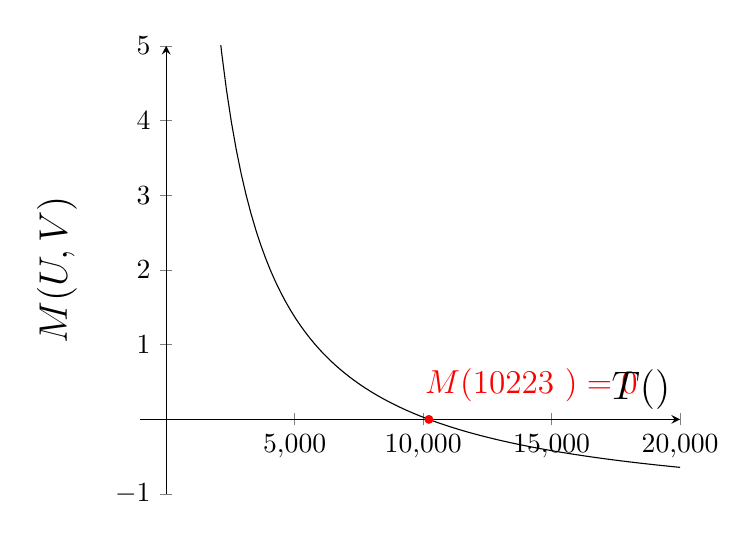
\begin{tikzpicture}
        \begin{axis}[axis lines = middle,
            xmin = -1000,
            xmax = 20000,
            ymin = -1,
            ymax = 5,
            ylabel = {\Large $M(U,V)$},
            ylabel style={at={(axis description cs:-0.1,.5)},rotate=90,anchor=south},
            xlabel = {\Large $T(\unit{\kelvin})$},
            ytick distance = 1,
            xtick distance = 5000,
            scaled x ticks = false,]
        
        \addplot [color = black, domain = 1000:20000, samples = 100] {13426.0958156/x - 1.31332249004};
        
        \node[color = red, anchor = south west] at (9700,0.1) {\large $M(10223\ \unit{\kelvin}) = 0$};
        
        \draw [red, fill = red] (10223,0) ellipse [x radius = 150, y radius = 0.052];
        
        \end{axis}
        \end{tikzpicture}
        
    \caption{Graph of $M(U,V)$ \emph{vs} $T$, for the relation \ref{eq:nice}}
\label{fig:graph2}
\end{figure}

\ut{B.5} From the graph in Figure \ref{fig:graph3}, we find that $M(U,V) = 0$ for $T \approx \num{10220}$~K. Notice that for any $T > \num{10220}$~K, the value of $M(U,V) < 0$, which indicates that the magnitude of the body in the ultraviolet band is greater than in the visible band. This means that most of the emitted radiation intensity is concentrated near blue and violet, giving the body a bluish coloration.

On the other hand, for lower temperatures ($T < \num{10220}$~K), the magnitude in the visible band is greater than in the ultraviolet, which means the body appears more reddish.

From the analysis of the graph, the Sun’s UV color index can be determined as $M_\odot(U,V) \approx 1.07$.

\begin{figure}[htpb]
    \centering
    \pgfplotsset{width = 15 cm}
    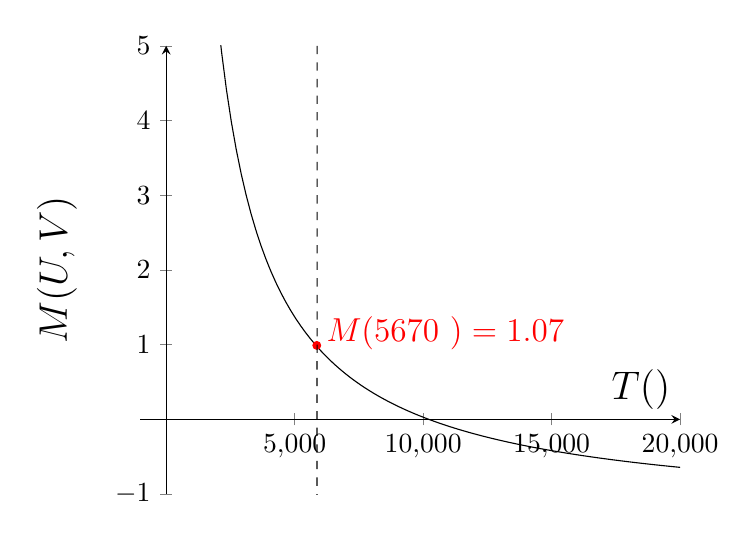
\begin{tikzpicture}
    \begin{axis}[axis lines = middle,
        xmin = -1000,
        xmax = 20000,
        ymin = -1,
        ymax = 5,
        ylabel = {\Large $M(U,V)$},
        ylabel style={at={(axis description cs:-0.1,.5)},rotate=90,anchor=south},
        xlabel = {\Large $T(\unit{\kelvin})$},
        ytick distance = 1,
        xtick distance = 5000,
        scaled x ticks = false,]

    \addplot [color = black, domain = 1000:20000, samples = 100] {13426.0958156/x - 1.31332249004};

    \draw [red, fill = red] (5860,0.99) ellipse [x radius = 150, y radius = 0.052];

    \node[color = red, anchor = south west] at (5860,0.8) {\large $M(5670\ \unit{\kelvin}) = 1.07$};

    \addplot[color = black, domain = 5860:5880, dashed]{x-5870};

    \end{axis}
    \end{tikzpicture}

    \caption{Graph of $M(U,V)$ \emph{vs} $T$, for the relation \ref{eq:nice} and the value of $M(5670\ \unit{\kelvin})$}
    \label{fig:graph3}
\end{figure}

    \clearpage
    \fi
\end{document}

    
